\documentclass{standalone}
\usepackage{tikz}
\usetikzlibrary{patterns, positioning}
\usepackage[sfdefault]{ClearSans} %% option 'sfdefault' activates Clear Sans as the default text font
\usepackage[T1]{fontenc}

\begin{document}
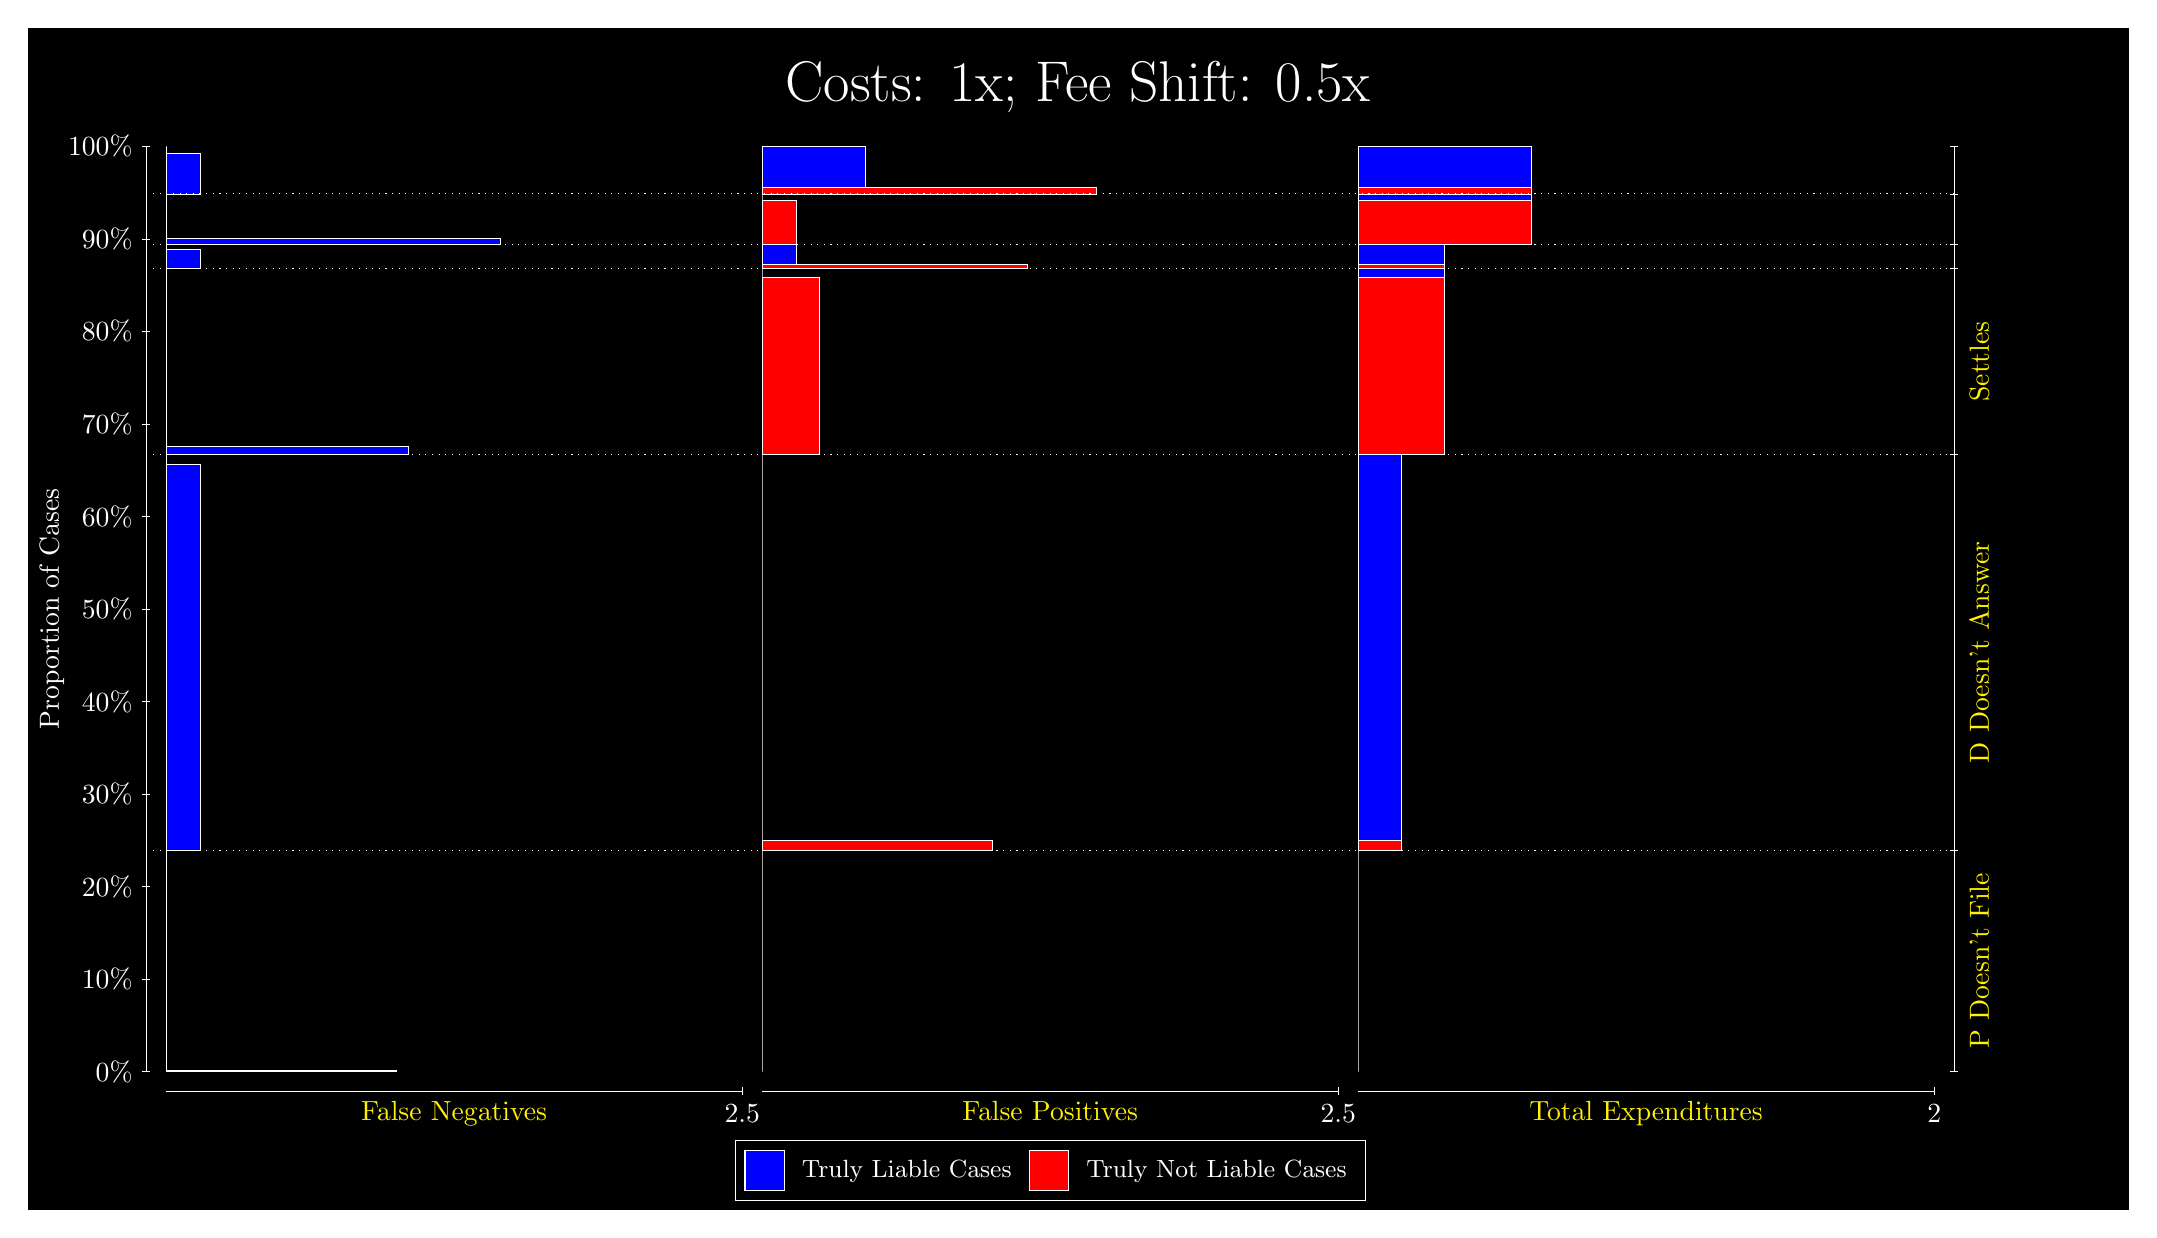
\begin{tikzpicture}
\draw[fill=black] (0,0) rectangle (26.667,15);
\draw[text=white] (0,13.5) rectangle (26.667,15) node[midway] {\huge Costs: 1x; Fee Shift: 0.5x};
\draw[white, very thin] (1.5,1.75) -- (1.5,13.5);
\node[rotate=90, text=white, anchor=center] at (0.3, 7.625) {Proportion of Cases};
\draw[white, very thin] (1.45,1.75) -- (1.55,1.75);
\node[text=white, anchor=east] at (1.45, 1.75) {0\%};
\draw[white, very thin] (1.45,2.925) -- (1.55,2.925);
\node[text=white, anchor=east] at (1.45, 2.925) {10\%};
\draw[white, very thin] (1.45,4.1) -- (1.55,4.1);
\node[text=white, anchor=east] at (1.45, 4.1) {20\%};
\draw[white, very thin] (1.45,5.275) -- (1.55,5.275);
\node[text=white, anchor=east] at (1.45, 5.275) {30\%};
\draw[white, very thin] (1.45,6.45) -- (1.55,6.45);
\node[text=white, anchor=east] at (1.45, 6.45) {40\%};
\draw[white, very thin] (1.45,7.625) -- (1.55,7.625);
\node[text=white, anchor=east] at (1.45, 7.625) {50\%};
\draw[white, very thin] (1.45,8.8) -- (1.55,8.8);
\node[text=white, anchor=east] at (1.45, 8.8) {60\%};
\draw[white, very thin] (1.45,9.975) -- (1.55,9.975);
\node[text=white, anchor=east] at (1.45, 9.975) {70\%};
\draw[white, very thin] (1.45,11.15) -- (1.55,11.15);
\node[text=white, anchor=east] at (1.45, 11.15) {80\%};
\draw[white, very thin] (1.45,12.325) -- (1.55,12.325);
\node[text=white, anchor=east] at (1.45, 12.325) {90\%};
\draw[white, very thin] (1.45,13.5) -- (1.55,13.5);
\node[text=white, anchor=east] at (1.45, 13.5) {100\%};

\draw[white, very thin] (24.457,1.75) -- (24.457,13.5);
\draw[white, very thin] (24.407,1.75) -- (24.507,1.75);
\node[anchor=west] at (24.407, 1.75) {};
\draw[white, very thin] (24.407,4.5581) -- (24.507,4.5581);
\node[anchor=west] at (24.407, 4.5581) {};
\draw[white, very thin] (24.407,9.5881) -- (24.507,9.5881);
\node[anchor=west] at (24.407, 9.5881) {};
\draw[white, very thin] (24.407,11.945) -- (24.507,11.945);
\node[anchor=west] at (24.407, 11.945) {};
\draw[white, very thin] (24.407,12.25) -- (24.507,12.25);
\node[anchor=west] at (24.407, 12.25) {};
\draw[white, very thin] (24.407,12.897) -- (24.507,12.897);
\node[anchor=west] at (24.407, 12.897) {};
\draw[white, very thin] (24.407,13.5) -- (24.507,13.5);
\node[anchor=west] at (24.407, 13.5) {};

\draw[white, very thin, fill=blue] (1.75,1.75) rectangle (4.6775,1.7689);
\draw[white, very thin, fill=red] (1.75,1.7689) rectangle (1.75,4.5581);
\draw[white, very thin, fill=blue] (1.75,4.5581) rectangle (2.1891,9.4598);
\draw[white, very thin, fill=red] (1.75,9.4598) rectangle (1.75,9.5881);
\draw[white, very thin, fill=blue] (1.75,9.5881) rectangle (4.8239,9.6929);
\draw[white, very thin, fill=red] (1.75,9.6929) rectangle (1.75,11.945);
\draw[white, very thin, fill=blue] (1.75,11.945) rectangle (2.1891,12.196);
\draw[white, very thin, fill=red] (1.75,12.196) rectangle (1.75,12.25);
\draw[white, very thin, fill=blue] (1.75,12.25) rectangle (5.9949,12.328);
\draw[white, very thin, fill=red] (1.75,12.328) rectangle (1.75,12.897);
\draw[white, very thin, fill=blue] (1.75,12.897) rectangle (2.1891,13.418);
\draw[white, very thin, fill=red] (1.75,13.418) rectangle (1.75,13.5);
\draw[white, very thin, fill=red] (9.3189,1.75) rectangle (9.3189,4.5393);
\draw[white, very thin, fill=blue] (9.3189,4.5393) rectangle (9.3189,4.5581);
\draw[white, very thin, fill=red] (9.3189,4.5581) rectangle (12.246,4.6864);
\draw[white, very thin, fill=blue] (9.3189,4.6864) rectangle (9.3189,9.5881);
\draw[white, very thin, fill=red] (9.3189,9.5881) rectangle (10.051,11.84);
\draw[white, very thin, fill=blue] (9.3189,11.84) rectangle (9.3189,11.945);
\draw[white, very thin, fill=red] (9.3189,11.945) rectangle (12.686,11.999);
\draw[white, very thin, fill=blue] (9.3189,11.999) rectangle (9.758,12.25);
\draw[white, very thin, fill=red] (9.3189,12.25) rectangle (9.758,12.819);
\draw[white, very thin, fill=blue] (9.3189,12.819) rectangle (9.3189,12.897);
\draw[white, very thin, fill=red] (9.3189,12.897) rectangle (13.564,12.979);
\draw[white, very thin, fill=blue] (9.3189,12.979) rectangle (10.636,13.5);
\draw[white, very thin, fill=red] (16.888,1.75) rectangle (16.888,4.5393);
\draw[white, very thin, fill=blue] (16.888,4.5393) rectangle (16.888,4.5581);
\draw[white, very thin, fill=red] (16.888,4.5581) rectangle (17.437,4.6864);
\draw[white, very thin, fill=blue] (16.888,4.6864) rectangle (17.437,9.5881);
\draw[white, very thin, fill=red] (16.888,9.5881) rectangle (17.986,11.84);
\draw[white, very thin, fill=blue] (16.888,11.84) rectangle (17.986,11.945);
\draw[white, very thin, fill=red] (16.888,11.945) rectangle (17.986,11.999);
\draw[white, very thin, fill=blue] (16.888,11.999) rectangle (17.986,12.25);
\draw[white, very thin, fill=red] (16.888,12.25) rectangle (19.083,12.819);
\draw[white, very thin, fill=blue] (16.888,12.819) rectangle (19.083,12.897);
\draw[white, very thin, fill=red] (16.888,12.897) rectangle (19.083,12.979);
\draw[white, very thin, fill=blue] (16.888,12.979) rectangle (19.083,13.5);
\draw[white, dotted] (1.5,4.5581) -- (24.457,4.5581);
\draw[white, dotted] (1.5,9.5881) -- (24.457,9.5881);
\draw[white, dotted] (1.5,11.945) -- (24.457,11.945);
\draw[white, dotted] (1.5,12.25) -- (24.457,12.25);
\draw[white, dotted] (1.5,12.897) -- (24.457,12.897);
\draw[white, very thin] (1.75,1.5) -- (9.0689,1.5);
\node[text=yellow, anchor=north] at (5.4094, 1.5) {False Negatives};
\draw[white, very thin] (9.0689,1.45) -- (9.0689,1.55);
\node[text=white, anchor=north] at (9.0689, 1.45) {2.5};

\draw[white, very thin] (9.3189,1.5) -- (16.638,1.5);
\node[text=yellow, anchor=north] at (12.978, 1.5) {False Positives};
\draw[white, very thin] (16.638,1.45) -- (16.638,1.55);
\node[text=white, anchor=north] at (16.638, 1.45) {2.5};

\draw[white, very thin] (16.888,1.5) -- (24.207,1.5);
\node[text=yellow, anchor=north] at (20.547, 1.5) {Total Expenditures};
\draw[white, very thin] (24.207,1.45) -- (24.207,1.55);
\node[text=white, anchor=north] at (24.207, 1.45) {2};

\node[text=yellow, centered, rotate=90] at (24.777, 3.1541) {P Doesn't File};
\node[text=yellow, centered, rotate=90] at (24.777, 7.0731) {D Doesn't Answer};
\node[text=yellow, centered, rotate=90] at (24.777, 10.767) {Settles};




\draw (12.978300999999998,1.5) node[draw=none] (baseCoordinate) {};
\begin{scope}[align=center]
        \matrix[scale=0.5, draw=white, below=0.5cm of baseCoordinate, nodes={draw}, column sep=0.1cm]{
            \node[rectangle, draw, minimum width=0.5cm, minimum height=0.5cm, fill=blue] {}; &
            \node[draw=none, font=\small, text=white] (B) {Truly Liable Cases}; &
            \node[rectangle, draw, minimum width=0.5cm, minimum height=0.5cm, fill=red] {}; &
            \node[draw=none, font=\small, text=white] (B) {Truly Not Liable Cases}; \\
            };
\end{scope}

\end{tikzpicture}
\end{document}